\subsection{Effect of the supply regularization strengths}

\begin{frame}[t]{Effect of supply regularization on the APF point}{}
    \onslide*<1-4>{
    All else fixed, what happens to \(\APFPoint\) when
    \(\XEDRegs \in \left\{0,10^{-4},1\right\} \times \left\{0,10^{-4},1\right\}\)?
    }
    \onslide*<2>{
    \begin{figure} 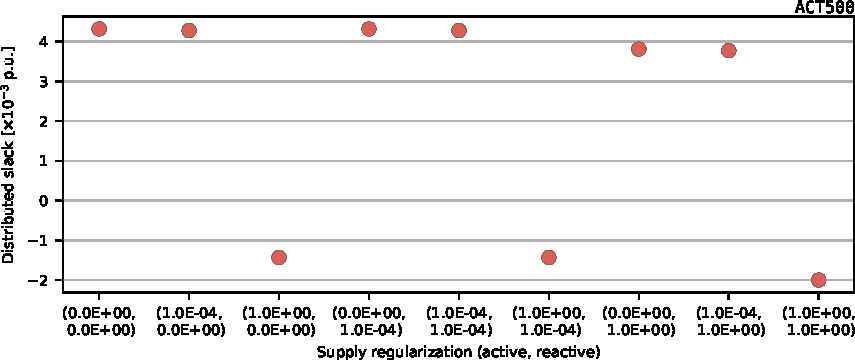
\includegraphics[width=0.95\textwidth]{trick_ACT500.pdf} \end{figure}
    }
    \onslide*<3>{
    \begin{figure} 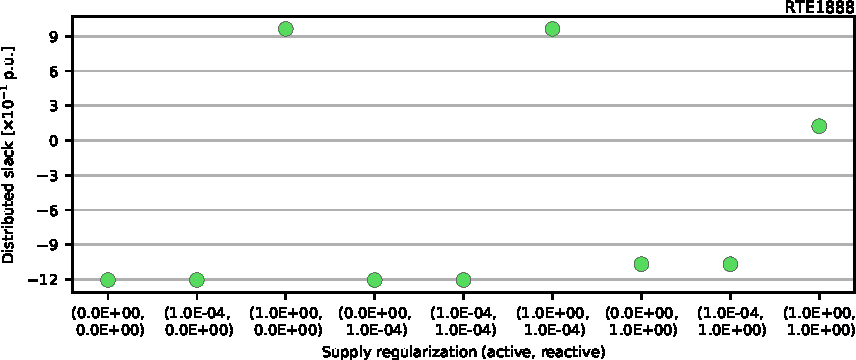
\includegraphics[width=0.95\textwidth]{trick_RTE1888.pdf} \end{figure}
    }
    \onslide*<4>{
    \begin{figure} 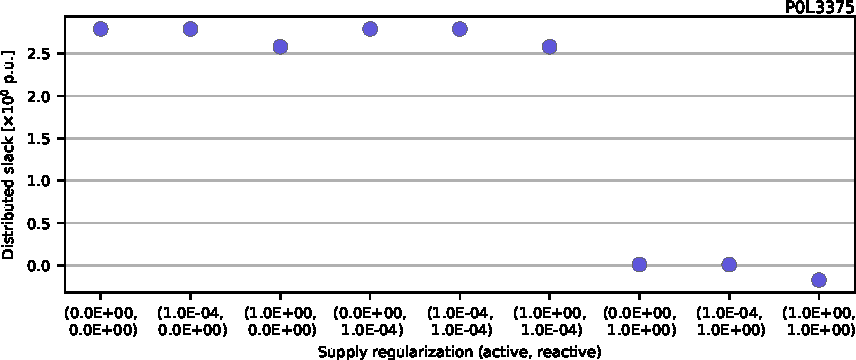
\includegraphics[width=0.95\textwidth]{trick_POL3375.pdf} \end{figure}
    }

    \begin{block}<5->{Quadrimodal effect}
        The APF point \(\APFPoint\) will be {\color{CornellRed}in one of four neighbourhoods}
        in the upcoming-dispatch PFM.
    \end{block}

    \begin{overlayarea}{\textwidth}{\textheight}
    \begin{onlyenv}<6>
    Consider \XED in 1D:
    minimize \(\AbsVal*{x} + \mu\AbsVal*{x-1}\) s.t. \(-3 \leq x \leq 3\), where \(\mu \geq 0\)
    \begin{figure} 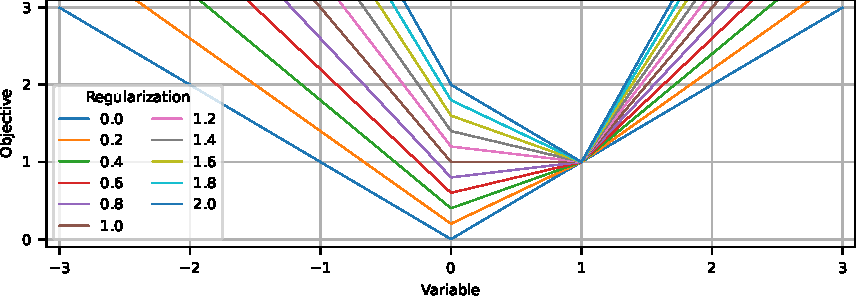
\includegraphics[width=0.95\textwidth]{1d-apf1.pdf} \end{figure}
    \end{onlyenv}

    \begin{onlyenv}<7>
    \begin{corollary}[Big-\(\mu\) trick for finding four APF points]
        Regularizing \XED with
        {\color{CornellRed}
        \(\XEDRegs \in \left\{0,\mu\right\} \times \left\{0,\mu\right\}\),
        for some \(\mu \gg 0\)},
        yields four \(\SupInjs\)'s,
        and, by \APFE, four \(\PFEVars\)'s.
        These {\color{CornellRed}four independent APF instances} can be run in parallel.
    \end{corollary}
    \end{onlyenv}
    \end{overlayarea}
\end{frame}
